\documentclass[12pt]{article}
\usepackage{geometry}
\usepackage{setspace}
\usepackage{graphicx}
\usepackage{booktabs}
\usepackage{float}
\usepackage[hidelinks]{hyperref}
\usepackage{amsmath}
\usepackage{amssymb}
\usepackage[utf8]{inputenc}
\usepackage{listings}
\usepackage{xcolor}
\usepackage{array}
\usepackage{tocloft}
\geometry{margin=1in}
\setstretch{1.15}

\lstset{
	language=Python,
	basicstyle=\ttfamily\footnotesize,
	backgroundcolor=\color{gray!10},
	frame=single,
	breaklines=true,
	breakatwhitespace=false,
	numbers=left,
	numberstyle=\tiny\color{gray},
	numbersep=5pt,
	showstringspaces=false,
	tabsize=4,
	captionpos=b,
	keywordstyle=\color{blue!70},
	stringstyle=\color{red!60},
	commentstyle=\color{green!50!black},
	morekeywords={as, True, False, None}
}

% ---- Custom List of Equations ----
\newcommand{\listequationsname}{List of Equations}
\newlistof{myequations}{equ}{\listequationsname}
\newcommand{\myequation}[1]{%
	\addcontentsline{equ}{myequations}{\protect\numberline{\theequation}#1}%
}

\begin{document}

% =====================================================================
% TITLE PAGE
% =====================================================================
\pagenumbering{roman}
\begin{titlepage}
	\centering
	\vspace*{2cm}

	{\Huge \textbf{EE627A Midterm}}\\[0.5cm]
	{\LARGE Heuristic-Based Music Recommendation}\\[2.5cm]

	{\Large \textbf{Jude Eschete}}\\[1cm]

	{\large
		\textbf{Course:} EE627A --- Data Acquisition and Processing~I: Big Data\\[0.3cm]
		\textbf{Instructor:} Prof.\ Rensheng Wang\\[0.3cm]
		\textbf{Semester:} Spring 2026\\[0.3cm]
		\textbf{Date:} \today
	}

	\vfill
\end{titlepage}

% =====================================================================
% TABLE OF CONTENTS, LIST OF FIGURES, LIST OF EQUATIONS
% =====================================================================
\newpage
\tableofcontents

\newpage
\listoffigures
\listoftables
\listofmyequations

% =====================================================================
\newpage
\pagenumbering{arabic}
\section{Part 1: Heuristic-Based Music Recommendation}
% =====================================================================

\subsection{Objective}

The goal is to develop a rule-based recommendation system for the Yahoo Music dataset. For each of 20,000 test users, the system is given six candidate tracks and must label exactly three as ``1'' (Recommend) and three as ``0'' (Do Not Recommend). The system is evaluated by AUC-ROC on the Kaggle leaderboard.

\subsection{Dataset Overview}

The Yahoo Music dataset stores music data in a hierarchical structure:

\begin{center}
\textbf{Track} $\rightarrow$ \textbf{Album} $\rightarrow$ \textbf{Artist} $\rightarrow$ \textbf{Genre(s)}
\end{center}

Users rate items across all hierarchy levels on a scale of 0--100. The training set contains ratings for tracks, albums, artists, and genres in a single flat ID space.

\begin{table}[H]
	\centering
	\caption{Dataset statistics.}\label{tab:dataset}
	\begin{tabular}{lr}
		\toprule
		\textbf{Property} & \textbf{Value} \\
		\midrule
		Training users          & 49,204 \\
		Total ratings           & 12,403,575 \\
		Tracks in metadata      & 224,041 \\
		Albums in metadata      & 52,829 \\
		Test users              & 20,000 \\
		Candidates per user     & 6 \\
		Total test candidates   & 120,000 \\
		\bottomrule
	\end{tabular}
\end{table}

%----------------------------------------------------------------------
\newpage
\subsection{Part 1.a: Feature Engineering \& Statistical Aggregation}
%----------------------------------------------------------------------

\subsubsection{Methodology}

For each candidate track, the system looks up the track's hierarchy (Album ID, Artist ID, and Genre IDs) from \texttt{trackData2.txt}, then searches the test user's training history for direct ratings of those hierarchy items.

The resulting feature vector for each (user, candidate-track) pair contains:

\begin{itemize}
	\item \textbf{Album Score}: The user's historical rating for the track's album (0 if not rated).
	\item \textbf{Artist Score}: The user's historical rating for the track's artist (0 if not rated).
	\item \textbf{Genre Statistics}: Computed over all of the track's genres that the user has rated:
	\begin{itemize}
		\item \textbf{Count}: Number of the track's genres rated by the user.
		\item \textbf{Maximum}: Highest rating among matched genres.
		\item \textbf{Minimum}: Lowest rating among matched genres.
		\item \textbf{Mean}: Average rating across matched genres.
		\item \textbf{Variance}: Variance of ratings across matched genres.
		\item \textbf{Sum}: Total of ratings across matched genres.
	\end{itemize}
	\item \textbf{Has Album / Has Artist}: Binary flags indicating whether the user has rated the album or artist at all.
\end{itemize}

\subsubsection{Data Sparsity Analysis}

A critical observation is that the training data is sparse at the hierarchy level. Not every user has rated the album, artist, or genres of every candidate track.

\begin{table}[H]
	\centering
	\caption{Feature coverage across all 120,000 test candidates.}\label{tab:sparsity}
	\begin{tabular}{lrr}
		\toprule
		\textbf{Feature} & \textbf{Count Present} & \textbf{Coverage (\%)} \\
		\midrule
		Album rating     & 34,264  & 28.6\% \\
		Artist rating    & 51,904  & 43.3\% \\
		$\geq$1 Genre rating & 58,223 & 48.5\% \\
		\midrule
		Avg.\ genre matches per candidate & \multicolumn{2}{c}{0.70} \\
		\bottomrule
	\end{tabular}
\end{table}

This sparsity directly influences the strategy design: any heuristic that relies solely on album scores will have no information for 71.4\% of candidates. Artist and genre signals provide broader coverage and are essential for discriminating among candidates.

\subsubsection{Feature Vector Example -- User 199810}

\begin{table}[H]
	\centering
	\caption{Feature vectors for the first test user (User 199810).}\label{tab:example}
	\footnotesize
	\begin{tabular}{r r r r r r r r r r}
		\toprule
		\textbf{TrackID} & \textbf{AlbumID} & \textbf{ArtistID} & \textbf{AlbScr} & \textbf{ArtScr} & \textbf{G\_Cnt} & \textbf{G\_Max} & \textbf{G\_Min} & \textbf{G\_Mean} & \textbf{G\_Var} \\
		\midrule
		208019 & 209288 & None & 0  & 0  & 0 & 0  & 0  & 0.0  & 0.0  \\
		74139  & 277282 & 271146 & 0  & 0  & 1 & 80 & 80 & 80.0 & 0.0  \\
		9903   & None   & None   & 0  & 0  & 0 & 0  & 0  & 0.0  & 0.0  \\
		242681 & 190640 & 244574 & 0  & 0  & 0 & 0  & 0  & 0.0  & 0.0  \\
		18515  & 146344 & 33168  & 0  & 70 & 0 & 0  & 0  & 0.0  & 0.0  \\
		105760 & 93458  & 11616  & 0  & 90 & 2 & 80 & 80 & 80.0 & 0.0  \\
		\bottomrule
	\end{tabular}
\end{table}

For User 199810, only three of six candidates have any training signal. Tracks 74139, 18515, and 105760 have artist and/or genre matches, while the remaining three tracks have no historical evidence. All three strategies correctly recommend the three tracks with non-zero feature values.

%----------------------------------------------------------------------
\newpage
\subsection{Part 1.b: Decision Logic \& Rule Definition}
%----------------------------------------------------------------------

Three heuristic strategies were implemented, each defining a composite score to rank the six candidates. The top three by score are recommended.

\subsubsection{Strategy 1: Maximum Genre Score}

\begin{equation}
	\text{Score} = 0.30 \times \text{AlbumScore} + 0.20 \times \text{ArtistScore} + 0.50 \times \text{GenreMax}
\end{equation}
\myequation{Strategy 1: Maximum Genre Score}

\textbf{Rationale:} Genre preference is a fundamental taste indicator. If a user gives a high rating to \emph{any} genre associated with a track, the track is likely to resonate with that user. The maximum (rather than mean) captures the ``best-case'' genre alignment and avoids dilution from low-rated secondary genres. Album and artist scores provide additional specificity.

\subsubsection{Strategy 2: Weighted Average}

\begin{equation}
	\text{Score} = 0.40 \times \text{AlbumScore} + 0.35 \times \text{ArtistScore} + 0.25 \times \text{GenreMean}
\end{equation}
\myequation{Strategy 2: Weighted Average}

\textbf{Rationale:} This strategy balances all three hierarchy levels with the strongest weight on the album (the most granular personalized signal, since the same album implies high content similarity), followed by artist affinity, and complemented by the user's average genre preference across all of the track's genres.

\subsubsection{Strategy 3: Evidence-Weighted Composite}

\begin{equation}
	\text{Score} = \text{HasAlbum} \times \text{AlbumScore} + \text{HasArtist} \times \text{ArtistScore} + \frac{\text{GenreCount} \times \text{GenreMean}}{10}
\end{equation}
\myequation{Strategy 3: Evidence-Weighted Composite}

\textbf{Rationale:} This strategy explicitly addresses data sparsity. A zero album score for an un-rated album is absence-of-evidence, not evidence-of-absence. The binary flags (\texttt{HasAlbum}, \texttt{HasArtist}) ensure that only \emph{actually rated} hierarchy items contribute to the score. Genre breadth (count $\times$ mean) rewards tracks where the user has interacted with many of the track's genres, providing stronger cumulative evidence.

\subsubsection{Cross-Strategy Agreement}

\begin{table}[H]
	\centering
	\caption{Pairwise agreement between strategies (out of 120,000 predictions).}\label{tab:agreement}
	\begin{tabular}{lrr}
		\toprule
		\textbf{Comparison} & \textbf{Agreement} & \textbf{Rate} \\
		\midrule
		MaxGenre vs.\ WeightedAvg    & 113,428 & 94.5\% \\
		MaxGenre vs.\ Evidence       & 111,722 & 93.1\% \\
		WeightedAvg vs.\ Evidence    & 117,138 & 97.6\% \\
		\bottomrule
	\end{tabular}
\end{table}

The strategies agree on 93--98\% of predictions, indicating that the underlying signals (album, artist, genre) are consistent. The remaining divergence comes from edge cases where sparsity handling or genre aggregation (max vs.\ mean) shifts the ranking of borderline candidates.

\subsection{Python Implementation}

The complete Python implementation for Part~1 is presented in Appendix~\ref{app:code}. The code handles data parsing, feature engineering, the three heuristic strategies, ranking, and Kaggle submission generation.

%----------------------------------------------------------------------
\newpage
\subsection{Part 1 Results}
%----------------------------------------------------------------------

\subsubsection{Submission Output}

Each strategy produces a Kaggle-format CSV with 120,000 rows (20,000 users $\times$ 6 candidates). Exactly 60,000 predictions are labeled ``1'' (recommend) and 60,000 labeled ``0'' (do not recommend), satisfying the constraint of 3 recommendations per user.

\subsubsection{Kaggle Leaderboard Results}

\begin{figure}[H]
	\centering
	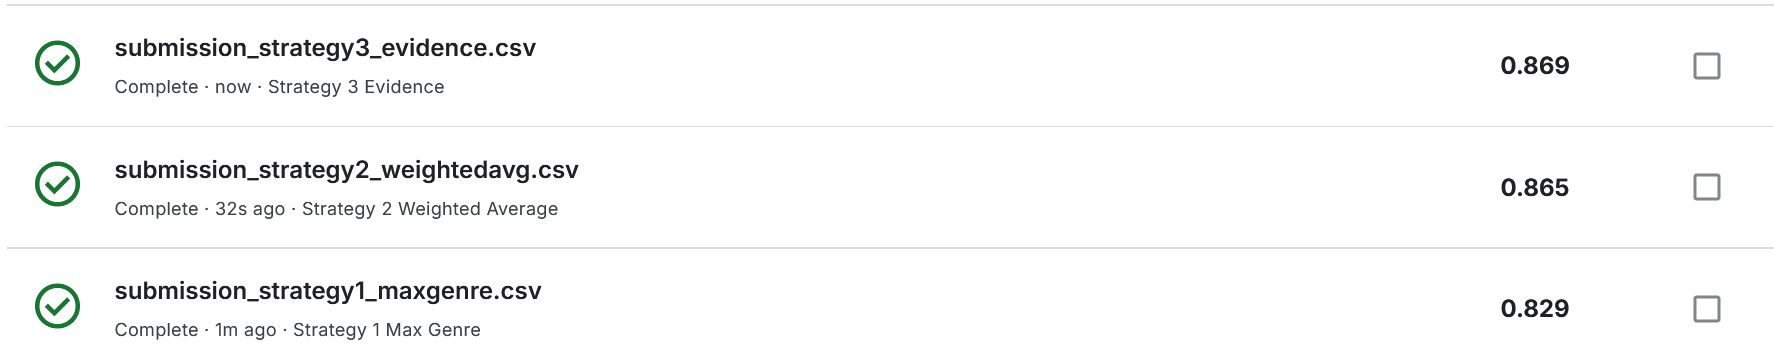
\includegraphics[width=0.85\textwidth]{images/part1Scores.png}
	\caption{Kaggle AUC-ROC scores for the three Part 1 strategies.}\label{fig:part1-kaggle}
\end{figure}

\begin{table}[H]
	\centering
	\caption{Part 1 Kaggle AUC-ROC comparison.}\label{tab:part1-kaggle}
	\begin{tabular}{llc}
		\toprule
		\textbf{Strategy} & \textbf{Scoring Rule} & \textbf{AUC-ROC} \\
		\midrule
		S1: Max Genre Score   & $0.30 \cdot \text{album} + 0.20 \cdot \text{artist} + 0.50 \cdot \text{genre\_max}$ & 0.829 \\
		S2: Weighted Average  & $0.40 \cdot \text{album} + 0.35 \cdot \text{artist} + 0.25 \cdot \text{genre\_mean}$ & 0.865 \\
		S3: Evidence-Weighted & $\text{has\_alb} \cdot \text{album} + \text{has\_art} \cdot \text{artist} + \frac{\text{g\_cnt} \cdot \text{g\_mean}}{10}$ & \textbf{0.869} \\
		\bottomrule
	\end{tabular}
\end{table}

\subsubsection{Part 1 Key Observations}

\begin{enumerate}
	\item \textbf{Evidence-Weighted wins (AUC = 0.869):} Strategy~3 outperforms the other two by explicitly addressing data sparsity. Rather than assigning a zero to un-rated albums/artists (which drags down scores for tracks the user may actually like), it only counts an item when the user has \emph{actually} rated it. This avoids penalizing tracks with missing data.

	\item \textbf{Weighted Average is a close second (AUC = 0.865):} Balancing album, artist, and mean genre scores is effective. The small gap to S3 suggests that the fixed zero-imputation for missing scores is only mildly harmful when all three hierarchy levels are combined.

	\item \textbf{Max Genre Score underperforms (AUC = 0.829):} Placing 50\% weight on a single genre's maximum rating is too aggressive. In a sparse dataset where only 48.5\% of candidates have any genre match, the genre\_max signal is zero for half the candidates, reducing discriminative power.

	\item \textbf{Severe data sparsity:} Only 28.6\% of candidates have a direct album rating, 43.3\% have an artist rating, and 48.5\% have at least one genre match. For roughly half of all candidates, the system has zero personalized features---motivating the cold-start strategies in Part~2.
\end{enumerate}

%----------------------------------------------------------------------
\newpage
\section{Part 2: Addressing the Cold Start Problem}
%----------------------------------------------------------------------

\subsection{Objective}

Part~1's data sparsity analysis revealed that 71.4\% of candidates lack a direct album rating, 56.7\% lack an artist rating, and 51.5\% have no genre match at all. Part~2 develops fallback strategies for these ``cold start'' scenarios.

%----------------------------------------------------------------------
\newpage
\subsection{Part 2.a: The Global Fallback}
%----------------------------------------------------------------------

\subsubsection{Strategy Design}

For candidates where the user has no direct rating for the album, artist, or genre, the system falls back to \textbf{global popularity}---the average rating for that item across \emph{all} users in the training set.

\textbf{Global popularity computation:} For each item ID in the training set, compute:
\begin{equation}
	\text{GlobalScore}(item) = \frac{\sum_{u \in \text{raters}(item)} r_{u,item}}{|\text{raters}(item)|}
\end{equation}
\myequation{Global Popularity Score}

This produces a global mean rating and rater count for every track, album, artist, and genre (295,799 items total).

\textbf{Feature imputation:} When a user has not rated a candidate's album (or artist, or genre), the system substitutes the global average rating for that item. This provides a non-personalized ``universally liked'' signal that is better than the zero-score default from Part~1.

\begin{table}[H]
	\centering
	\caption{Album score source breakdown with Global Fallback.}\label{tab:global-src}
	\begin{tabular}{lrr}
		\toprule
		\textbf{Source} & \textbf{Count} & \textbf{Percentage} \\
		\midrule
		Direct (user rated album)   & 34,264  & 28.6\% \\
		Global (avg.\ across users) & 77,164  & 64.3\% \\
		None (album ID unknown)     &  8,572  &  7.1\% \\
		\bottomrule
	\end{tabular}
\end{table}

Global imputation fills album scores for 64.3\% of candidates that had no direct rating. The remaining 7.1\% have an album ID of \texttt{None} in the track metadata, so no imputation is possible.

%----------------------------------------------------------------------
\newpage
\subsection{Part 2.b: Dig Deeper Search Logic}
%----------------------------------------------------------------------

\subsubsection{Strategy Design}

When a user has no direct rating for a candidate track's album, the system performs a ``Dig Deeper'' search: it looks for \textbf{sibling tracks}---other tracks that belong to the same album---that the user \emph{has} rated.

\textbf{The logic:} Given a candidate track $t$ with Album ID $a$:
\begin{enumerate}
	\item Build an index: album $\rightarrow$ [track IDs] from \texttt{trackData2.txt}
	\item If the user has not directly rated album $a$, find all tracks $\{t_1, t_2, \ldots\}$ that share album $a$
	\item Check which of those sibling tracks the user has rated in training
	\item If any exist, compute the proxy album score as:
\end{enumerate}

\begin{equation}
	\text{AlbumProxy}(u, a) = \frac{1}{|S|} \sum_{t_i \in S} r_{u, t_i}
	\quad \text{where } S = \{t_i \in \text{album}(a) \mid t_i \in \text{rated}(u)\}
\end{equation}
\myequation{Album Proxy via Sibling Tracks (Dig Deeper)}

The mean aggregation is chosen over the maximum because it provides a more robust estimate---a single high-rated sibling could be an outlier, while the average reflects the user's overall engagement with the album's content.

\subsubsection{Hierarchical Fallback Implementation}

The full pipeline follows this priority:
\begin{enumerate}
	\item \textbf{Primary:} Direct Album/Artist/Genre scores from user history
	\item \textbf{Secondary (Dig Deeper):} If album score is missing, compute mean sibling-track rating for that album
	\item \textbf{Tertiary (Global):} If no sibling tracks found, use the global average rating
\end{enumerate}

Artist and genre scores use a simpler two-level fallback (Direct $\rightarrow$ Global).

\subsection{Part 2 Python Implementation}

The Part~2 Python code---including the album-to-tracks index, global statistics computation, and the enhanced feature vector with hierarchical fallback---is presented in Appendix~\ref{app:code}.

%----------------------------------------------------------------------
\newpage
\subsection{Part 2 Impact Analysis}
%----------------------------------------------------------------------

\subsubsection{Fallback Source Distribution}

\begin{table}[H]
	\centering
	\caption{Album score source: Global-only vs.\ full Hierarchical fallback.}\label{tab:source-compare}
	\begin{tabular}{lrrrr}
		\toprule
		\textbf{Source} & \multicolumn{2}{c}{\textbf{Global Only}} & \multicolumn{2}{c}{\textbf{Hierarchical}} \\
		\cmidrule(lr){2-3} \cmidrule(lr){4-5}
		& Count & \% & Count & \% \\
		\midrule
		Direct     & 34,264 & 28.6 & 34,264 & 28.6 \\
		Dig Deeper &      0 &  0.0 &  5,678 &  4.7 \\
		Global     & 77,164 & 64.3 & 71,486 & 59.6 \\
		None       &  8,572 &  7.1 &  8,572 &  7.1 \\
		\bottomrule
	\end{tabular}
\end{table}

The Dig Deeper logic identified 5,678 candidates (4.7\%) where the user had not rated the album directly but \emph{had} rated sibling tracks in the same album. These candidates shifted from the less-personalized ``Global'' source to the more-personalized ``Dig Deeper'' proxy.

\subsubsection{Prediction Changes}

\begin{table}[H]
	\centering
	\caption{Prediction changes vs.\ Part 1 baseline (WeightedAvg strategy).}\label{tab:impact}
	\begin{tabular}{lrr}
		\toprule
		\textbf{Comparison} & \textbf{Changed} & \textbf{Rate} \\
		\midrule
		Part 1 vs.\ Global Only     & 24,472 & 20.4\% \\
		Part 1 vs.\ Hierarchical    & 24,362 & 20.3\% \\
		Global Only vs.\ Hierarchical & 2,374 &  2.0\% \\
		\bottomrule
	\end{tabular}
\end{table}

\subsubsection{Kaggle Leaderboard Results}

\begin{figure}[H]
	\centering
	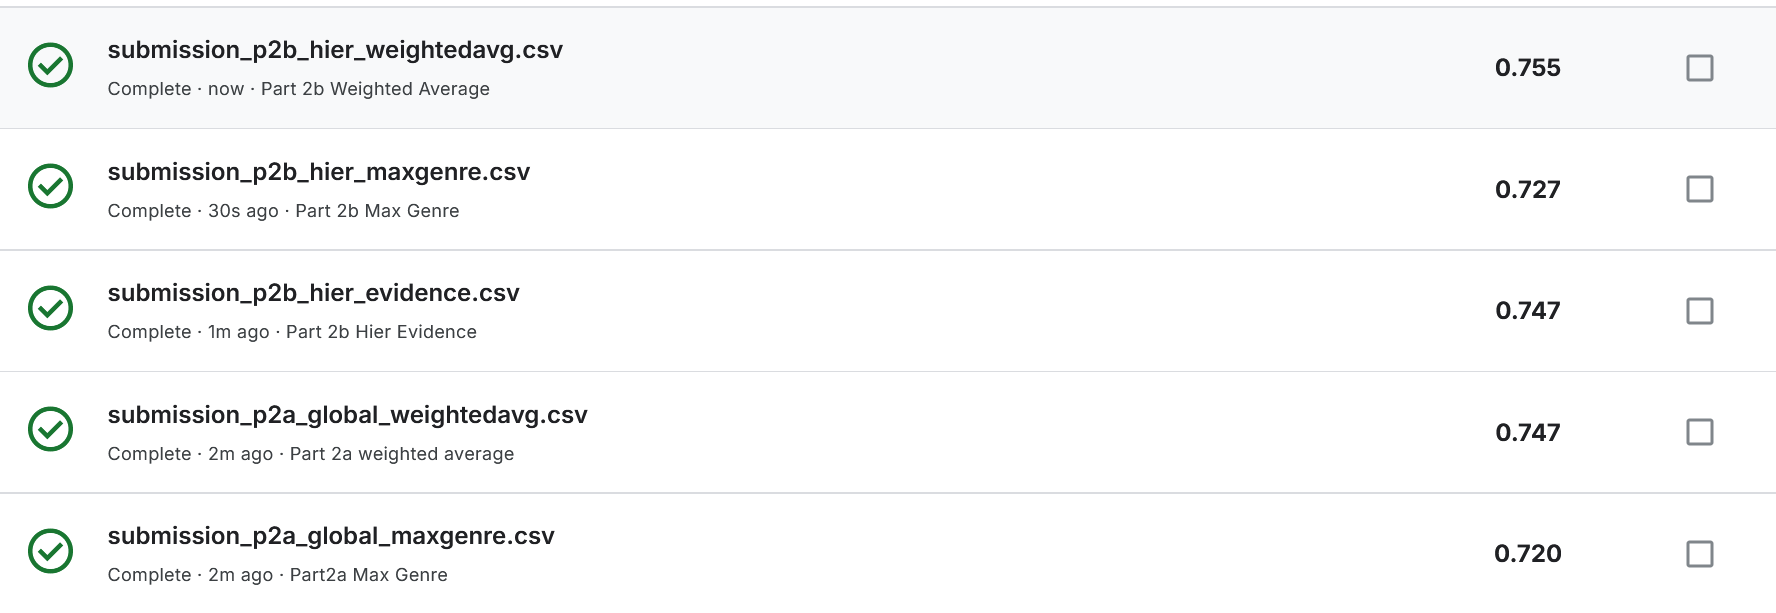
\includegraphics[width=0.85\textwidth]{images/part2Scores.png}
	\caption{Kaggle AUC-ROC scores for the Part 2 strategies.}\label{fig:part2-kaggle}
\end{figure}

\begin{table}[H]
	\centering
	\caption{Complete Kaggle AUC-ROC comparison: Part 1 vs.\ Part 2.}\label{tab:all-kaggle}
	\begin{tabular}{llcc}
		\toprule
		\textbf{Part} & \textbf{Strategy} & \textbf{AUC-ROC} & \textbf{$\Delta$ vs.\ Part 1} \\
		\midrule
		1  & S1: Max Genre Score      & 0.829 & --- \\
		1  & S2: Weighted Average     & 0.865 & --- \\
		1  & S3: Evidence-Weighted    & \textbf{0.869} & --- \\
		\midrule
		2a & Global + MaxGenre        & 0.720 & $-0.109$ \\
		2a & Global + WeightedAvg     & 0.747 & $-0.118$ \\
		\midrule
		2b & Hier + MaxGenre          & 0.727 & $-0.102$ \\
		2b & Hier + Evidence          & 0.747 & $-0.122$ \\
		2b & Hier + WeightedAvg       & 0.755 & $-0.110$ \\
		\bottomrule
	\end{tabular}
\end{table}

\subsubsection{Key Findings --- Why Fallback Scores Decreased}

A critical and instructive result: the Part~2 cold-start strategies \emph{decreased} AUC-ROC by 0.10--0.12 compared to Part~1. This is a well-documented phenomenon in recommender systems, and understanding \emph{why} is the central takeaway.

\begin{enumerate}
	\item \textbf{Global imputation introduces noise that drowns the personalized signal.}
	In Part~1, when a user has not rated an album, the album score is 0. This zero is not informative, but it is \emph{harmless}: candidates with actual user ratings naturally dominate the ranking, while unrated candidates tie at zero and are ranked arbitrarily among themselves. The personalized signal stays clean.

	In Part~2, replacing those zeros with global averages (typically in the 50--80 range) gives \emph{every} candidate a non-zero score. But these imputed scores are not personalized---they reflect crowd popularity, not individual taste. A track the user has never encountered can now outscore a track the user genuinely interacted with, purely because it is globally popular. This \textbf{dilutes the personalized signal} and degrades ranking quality.

	\item \textbf{Absence-of-evidence $\neq$ evidence-of-absence.}
	Part~1's Evidence-Weighted strategy (S3, AUC = 0.869) already handled this correctly: it only counts a score when the user \emph{actually} rated that hierarchy item, avoiding the ``zero penalty'' without introducing imputation noise. The Part~2 global fallback effectively undoes this advantage by treating ``not rated'' as ``rated at the global average,'' which is a stronger and less accurate assumption.

	\item \textbf{Dig Deeper provides a small relative lift within Part~2.}
	Comparing Part~2a (Global only) to Part~2b (Hierarchical), the Dig Deeper logic does improve scores slightly (e.g., WeightedAvg: 0.747 $\rightarrow$ 0.755, a +0.008 lift). This confirms that when sibling-track evidence exists, it is more predictive than the global average. However, the Dig Deeper rule only triggers for 4.7\% of candidates, so its impact is limited.

	\item \textbf{Data sparsity limits Dig Deeper's reach.}
	The Dig Deeper rule requires the user to have rated at least one other track in the same album---a rare condition in a dataset with 224,041 tracks spread across 31,141 albums. Only 5,678 of 120,000 candidates (4.7\%) met this condition. This extreme sparsity is the fundamental constraint on the strategy's effectiveness.

	\item \textbf{Lesson learned.}
	Naive feature imputation can be counterproductive in sparse recommendation settings. The optimal approach from Part~1 (Evidence-Weighted, AUC = 0.869) works precisely because it respects the distinction between ``no data'' and ``low preference.'' A more sophisticated cold-start strategy would need to impute selectively---e.g., only for users with truly zero features---rather than applying global averages uniformly across all missing values.
\end{enumerate}

%----------------------------------------------------------------------
\newpage
\section{All Submission Files}
%----------------------------------------------------------------------

\begin{table}[H]
	\centering
	\caption{Complete list of Kaggle submission files.}\label{tab:all-subs}
	\footnotesize
	\begin{tabular}{lllc}
		\toprule
		\textbf{Part} & \textbf{Strategy} & \textbf{File} & \textbf{AUC} \\
		\midrule
		1  & S1: Max Genre Score     & \texttt{submission\_strategy1\_maxgenre.csv}     & 0.829 \\
		1  & S2: Weighted Average    & \texttt{submission\_strategy2\_weightedavg.csv}  & 0.865 \\
		1  & S3: Evidence-Weighted   & \texttt{submission\_strategy3\_evidence.csv}     & \textbf{0.869} \\
		\midrule
		2a & Global + MaxGenre       & \texttt{submission\_p2a\_global\_maxgenre.csv}      & 0.720 \\
		2a & Global + WeightedAvg    & \texttt{submission\_p2a\_global\_weightedavg.csv}   & 0.747 \\
		\midrule
		2b & Hier + MaxGenre         & \texttt{submission\_p2b\_hier\_maxgenre.csv}        & 0.727 \\
		2b & Hier + Evidence         & \texttt{submission\_p2b\_hier\_evidence.csv}        & 0.747 \\
		2b & Hier + WeightedAvg      & \texttt{submission\_p2b\_hier\_weightedavg.csv}     & 0.755 \\
		\bottomrule
	\end{tabular}
\end{table}

% =====================================================================
\newpage
\appendix
\section{Python Source Code}\label{app:code}
% =====================================================================

The complete Python implementation is contained in a single script (\texttt{EE627\_Midterm.py}). The code is organized into data parsing, feature engineering, heuristic strategies, and the execution pipeline.

\subsection{Data Parsing}

\begin{lstlisting}[caption={Data parsing functions.}]
import os

SCRIPT_DIR = os.path.dirname(os.path.abspath(__file__))
DATA_DIR = os.path.join(SCRIPT_DIR, "..", "Homework 4", "Data")
TRAIN_FILE = os.path.join(DATA_DIR, "trainItem2.txt")
TEST_FILE  = os.path.join(DATA_DIR, "testItem2.txt")
TRACK_FILE = os.path.join(DATA_DIR, "trackData2.txt")
ALBUM_FILE = os.path.join(DATA_DIR, "albumData2.txt")
OUTPUT_DIR = SCRIPT_DIR


def parse_training(path):
    """Parse training file into {user_id: {item_id: rating}}.
    Format: UserID|NumItems header, then ItemID<TAB>Rating lines.
    Items can be tracks, albums, artists, or genres."""
    users = {}
    with open(path, "r") as f:
        uid = None
        for line in f:
            line = line.strip()
            if "|" in line:
                uid = int(line.split("|")[0])
                users[uid] = {}
            elif "\t" in line and uid is not None:
                parts = line.split("\t")
                users[uid][int(parts[0])] = int(parts[1])
    return users


def parse_tracks(path):
    """Parse trackData2.txt -> {tid: (album, artist, [genres])}."""
    tracks = {}
    with open(path, "r") as f:
        for line in f:
            parts = line.strip().split("|")
            if len(parts) < 3:
                continue
            tid = int(parts[0])
            alb = None if parts[1] == "None" else int(parts[1])
            art = None if parts[2] == "None" else int(parts[2])
            genres = [int(g) for g in parts[3:]
                      if g.strip() and g != "None"]
            tracks[tid] = (alb, art, genres)
    return tracks


def parse_test(path):
    """Parse testItem2.txt -> [(user_id, [track_ids])]."""
    test = []
    with open(path, "r") as f:
        uid, tids = None, []
        for line in f:
            line = line.strip()
            if "|" in line:
                if uid is not None:
                    test.append((uid, tids))
                uid = int(line.split("|")[0])
                tids = []
            elif line:
                tids.append(int(line))
        if uid is not None:
            test.append((uid, tids))
    return test
\end{lstlisting}

\subsection{Feature Engineering (Part 1)}

\begin{lstlisting}[caption={Feature engineering (Part 1.a).}]
def compute_feature_vector(user_ratings, track_meta, uid, tid):
    """Build feature vector for one (user, track) pair."""
    ratings = user_ratings.get(uid, {})
    alb_id, art_id, genre_ids = track_meta.get(
        tid, (None, None, []))

    # Album score
    if alb_id is not None and alb_id in ratings:
        album_score, has_album = ratings[alb_id], 1
    else:
        album_score, has_album = 0, 0

    # Artist score
    if art_id is not None and art_id in ratings:
        artist_score, has_artist = ratings[art_id], 1
    else:
        artist_score, has_artist = 0, 0

    # Genre statistics
    genre_scores = [ratings[g] for g in genre_ids
                    if g in ratings]
    n = len(genre_scores)
    if n > 0:
        g_max  = max(genre_scores)
        g_min  = min(genre_scores)
        g_mean = sum(genre_scores) / n
        g_var  = sum((s - g_mean)**2 for s in genre_scores) / n
        g_sum  = sum(genre_scores)
    else:
        g_max = g_min = g_sum = 0
        g_mean = g_var = 0.0

    return {
        "album_score": album_score,
        "artist_score": artist_score,
        "has_album": has_album,    "has_artist": has_artist,
        "genre_count": n,          "genre_max": g_max,
        "genre_min": g_min,        "genre_mean": g_mean,
        "genre_var": g_var,        "genre_sum": g_sum,
    }
\end{lstlisting}

\subsection{Heuristic Strategies (Part 1)}

\begin{lstlisting}[caption={Heuristic strategies (Part 1.b).}]
def strategy_max_genre(features_list):
    """Strategy 1: 0.30*album + 0.20*artist + 0.50*genre_max"""
    return [0.30 * f["album_score"]
            + 0.20 * f["artist_score"]
            + 0.50 * f["genre_max"]
            for f in features_list]


def strategy_weighted_avg(features_list):
    """Strategy 2: 0.40*album + 0.35*artist + 0.25*genre_mean"""
    return [0.40 * f["album_score"]
            + 0.35 * f["artist_score"]
            + 0.25 * f["genre_mean"]
            for f in features_list]


def strategy_evidence_weighted(features_list):
    """Strategy 3: has_album*album + has_artist*artist
       + genre_count*genre_mean/10"""
    return [f["has_album"] * f["album_score"]
            + f["has_artist"] * f["artist_score"]
            + f["genre_count"] * f["genre_mean"] / 10.0
            for f in features_list]
\end{lstlisting}

\subsection{Ranking and Submission Pipeline}

\begin{lstlisting}[caption={Ranking and submission pipeline.}]
def rank_top3(scores, track_ids):
    """Pick top-3 scored tracks as '1', rest as '0'."""
    paired = sorted(zip(scores, track_ids),
                    key=lambda x: x[0], reverse=True)
    top3 = set(tid for _, tid in paired[:3])
    return {tid: (1 if tid in top3 else 0)
            for tid in track_ids}


def write_submission(results, path):
    with open(path, "w") as f:
        f.write("TrackID,Predictor\n")
        for key, label in results:
            f.write(f"{key},{label}\n")


def run_strategy(user_ratings, track_meta, test_users,
                 strategy_fn, out_path):
    results = []
    for uid, candidates in test_users:
        feats  = [compute_feature_vector(
                      user_ratings, track_meta, uid, tid)
                  for tid in candidates]
        scores = strategy_fn(feats)
        recs   = rank_top3(scores, candidates)
        for tid in candidates:
            results.append((f"{uid}_{tid}", recs[tid]))
    write_submission(results, out_path)
    return results
\end{lstlisting}

\subsection{Main Entry Point (Part 1)}

\begin{lstlisting}[caption={Main entry point.}]
if __name__ == "__main__":
    user_ratings = parse_training(TRAIN_FILE)
    track_meta   = parse_tracks(TRACK_FILE)
    test_users   = parse_test(TEST_FILE)

    # Strategy 1: Max Genre Score
    run_strategy(user_ratings, track_meta, test_users,
        strategy_max_genre,
        os.path.join(OUTPUT_DIR,
            "submission_strategy1_maxgenre.csv"))

    # Strategy 2: Weighted Average
    run_strategy(user_ratings, track_meta, test_users,
        strategy_weighted_avg,
        os.path.join(OUTPUT_DIR,
            "submission_strategy2_weightedavg.csv"))

    # Strategy 3: Evidence-Weighted
    run_strategy(user_ratings, track_meta, test_users,
        strategy_evidence_weighted,
        os.path.join(OUTPUT_DIR,
            "submission_strategy3_evidence.csv"))
\end{lstlisting}

\subsection{Part 2: Cold-Start Extensions}

\begin{lstlisting}[caption={Album-to-tracks index and global statistics (Part 2 setup).}]
from collections import defaultdict

def build_album_to_tracks(track_meta):
    """Build {album_id: [track_ids]} for Dig Deeper."""
    album_tracks = defaultdict(list)
    for tid, (alb, _, _) in track_meta.items():
        if alb is not None:
            album_tracks[alb].append(tid)
    return dict(album_tracks)


def build_global_stats(user_ratings):
    """Global mean rating per item across all users.
    Returns {item_id: (mean_rating, num_raters)}."""
    item_sum = defaultdict(float)
    item_cnt = defaultdict(int)
    for _, ratings in user_ratings.items():
        for item_id, rating in ratings.items():
            item_sum[item_id] += rating
            item_cnt[item_id] += 1
    return {iid: (item_sum[iid] / item_cnt[iid],
                  item_cnt[iid])
            for iid in item_sum}
\end{lstlisting}

\begin{lstlisting}[caption={Enhanced feature vector with hierarchical fallback.}]
def compute_feature_vector_v2(user_ratings, track_meta,
        uid, tid, album_to_tracks, global_stats,
        use_dig_deeper=True, use_global=True):
    ratings = user_ratings.get(uid, {})
    alb_id, art_id, genre_ids = track_meta.get(
        tid, (None, None, []))

    # Album: Direct -> Dig Deeper -> Global
    album_score, has_album, album_source = 0, 0, "none"
    if alb_id is not None:
        if alb_id in ratings:
            album_score = ratings[alb_id]
            has_album, album_source = 1, "direct"
        elif use_dig_deeper:
            siblings = album_to_tracks.get(alb_id, [])
            sib_ratings = [ratings[st] for st in siblings
                           if st in ratings and st != tid]
            if sib_ratings:
                album_score = sum(sib_ratings)/len(sib_ratings)
                has_album, album_source = 1, "dig_deeper"
            elif use_global and alb_id in global_stats:
                album_score = global_stats[alb_id][0]
                has_album, album_source = 1, "global"
        elif use_global and alb_id in global_stats:
            album_score = global_stats[alb_id][0]
            has_album, album_source = 1, "global"

    # Artist: Direct -> Global
    artist_score, has_artist = 0, 0
    if art_id is not None:
        if art_id in ratings:
            artist_score, has_artist = ratings[art_id], 1
        elif use_global and art_id in global_stats:
            artist_score = global_stats[art_id][0]
            has_artist = 1

    # Genre: Direct -> Global (per genre)
    genre_scores = []
    for gid in genre_ids:
        if gid in ratings:
            genre_scores.append(ratings[gid])
        elif use_global and gid in global_stats:
            genre_scores.append(global_stats[gid][0])

    # ... compute genre stats as in Part 1 ...
\end{lstlisting}

\end{document}
